\begin{questions}

\question 在亚里士多德体系中,哪些物理量是绝对的?哪些物理量
是相对的?在牛顿体系中,哪些物理量是绝对的?哪些物理量是
相对的?

\question 变换关系式\eqref{eqn:02.03.06}是否只适用于$u$为常量的两个坐标间
的速度变换?

\question 试再举出一些有用的坐标变换。

\question 试举出一种相对于时间倒转变换为不变的运动。

\begin{wrapfigure}[10]{r}{12em}
    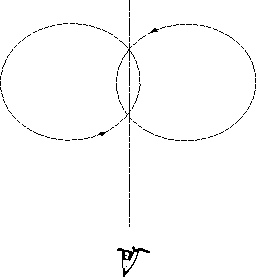
\includegraphics{figure/fig02.16}
    \caption{}
    \label{fig:02.16}
\end{wrapfigure}

\question 双星是一种天体,两颗星
绕它们共同的质心在一封闭的轨
道上绕行(图\ref{fig:02.16}),如果我们的
视线在轨道平面上,则双星中任
何一颗星有时向着我们运动,有
时离开我们运动。假使光速与光
源速度有关,可用速度合成公式
\eqref{eqn:02.03.06}。这样,我们将会看到什
么现象?

\question 如果地球总是以恒定的
速度运动,也没有自转,能探测到光行差效应吗?

\question 由于地球的周年运动引起的光行差效应,使得恒星的视位
置在一年之中绘出怎样的图形?
% 085.jpg
\clearpage
\question 在\ref{sec:02.07}~节中所述“运动钟的变慢”,是否是由于我们选用的雷达钟的特殊结构而引起的?
\end{questions}
